%%%%%%%%%%%%%%%%%%%%%%%%%%%%%%%%%%%%%%%%%
% University/School Laboratory Report
% LaTeX Template
% Version 3.1 (25/3/14)
%
% This template has been downloaded from:
% http://www.LaTeXTemplates.com
%
% Original author:
% Linux and Unix Users Group at Virginia Tech Wiki 
% (https://vtluug.org/wiki/Example_LaTeX_chem_lab_report)
%
% License:
% CC BY-NC-SA 3.0 (http://creativecommons.org/licenses/by-nc-sa/3.0/)
%
%%%%%%%%%%%%%%%%%%%%%%%%%%%%%%%%%%%%%%%%%

%----------------------------------------------------------------------------------------
%	PACKAGES AND DOCUMENT CONFIGURATIONS
%----------------------------------------------------------------------------------------

\documentclass{article}

\usepackage{polski}
\usepackage[utf8]{inputenc}
\usepackage{booktabs}
\usepackage{multirow}
\usepackage{caption}

\usepackage[version=3]{mhchem} % Package for chemical equation typesetting
\usepackage{siunitx} % Provides the \SI{}{} and \si{} command for typesetting SI units
\usepackage{graphicx} % Required for the inclusion of images
\usepackage{natbib} % Required to change bibliography style to APA
\usepackage{amsmath} % Required for some math elements 

\setlength\parindent{0pt} % Removes all indentation from paragraphs

\renewcommand{\labelenumi}{\alph{enumi}.} % Make numbering in the enumerate environment by letter rather than number (e.g. section 6)
\usepackage{color}

%\usepackage{times} % Uncomment to use the Times New Roman font

%----------------------------------------------------------------------------------------
%	DOCUMENT INFORMATION
%----------------------------------------------------------------------------------------

\title{Ćwiczenie nr 82: Efekt fotoelektryczny} % Title

\author{Rafał \textsc{Grabiański} i Zbigniew \textsc{Królikowski}} % Author name

\date{\today} % Date for the report

\addtolength{\oddsidemargin}{-.875in}
\addtolength{\evensidemargin}{-.875in}
\addtolength{\textwidth}{1.75in}
\addtolength{\topmargin}{-.875in}
\addtolength{\textheight}{1.75in}

\begin{document}

% Please add the following required packages to your document preamble:
% \usepackage{booktabs}
\begin{table}[h]
\begin{tabular}{@{}llllll@{}}
\toprule
\begin{tabular}[c]{@{}l@{}}Wydział:\\ \\ WIEiT\end{tabular}                                    & \multicolumn{2}{l}{\begin{tabular}[c]{@{}l@{}}Imię i nazwisko:\\ Rafał Grabiański\\ Zbigniew Królikowski\end{tabular}}                & \begin{tabular}[c]{@{}l@{}}Rok:\\ \\ II\end{tabular}            & \begin{tabular}[c]{@{}l@{}}Grupa:\\ \\ 7\end{tabular}              & \begin{tabular}[c]{@{}l@{}}Zespół:\\ \\ 7\end{tabular} \\ \midrule
\multicolumn{1}{|c|}{\begin{tabular}[c]{@{}c@{}}PRACOWNIA\\ FIZYCZNA\\ WFiIS AGH\end{tabular}} & \multicolumn{4}{l|}{Temat: Kriogenika}                                                                                                                                                                                                                                                  & \multicolumn{1}{l|}{Nr ćwiczenia: 113}                     \\ \midrule
\begin{tabular}[c]{@{}l@{}}Data wykonania:\\ \\ \\ 2.12.2014\end{tabular}                     & \begin{tabular}[c]{@{}l@{}}Data oddania:\\ \\ \\ 9.12.2014\end{tabular} & \begin{tabular}[c]{@{}l@{}}Zwrot do poprawy:\\ \\ \\ .\end{tabular} & \begin{tabular}[c]{@{}l@{}}Data oddania:\\ \\ \\ .\end{tabular} & \begin{tabular}[c]{@{}l@{}}Data zaliczenia:\\ \\ \\ .\end{tabular} & OCENA:                                                  \\ \bottomrule
\end{tabular}
\end{table}

%\maketitle % Insert the title, author and date

% If you wish to include an abstract, uncomment the lines below


%----------------------------------------------------------------------------------------
%	SECTION 1 - CEL ĆWICZENIA
%----------------------------------------------------------------------------------------

\section{Cel ćwiczenia}

Celem ćwiczenia było wyznaczenie ciepła parowania ciekłego azotu oraz zależności temperatury wrzenia od ciśnienia. Mieliśmy także dokonać obserwacji zestalenia ciekłego azotu przy obniżonym ciśnieniu i ustalić położenie punktu potrójnego.

% If you have more than one objective, uncomment the below:
%\begin{description}
%\item[First Objective] \hfill \\
%Objective 1 text
%\item[Second Objective] \hfill \\
%Objective 2 text
%\end{description}

 

%\clearpage

%----------------------------------------------------------------------------------------
%	SECTION 4
%----------------------------------------------------------------------------------------
\section{Wyniki pomiarów}

\begin{table}[htbp]
\centering
\begin{tabular}{|r|r|r|r|r|r|}
\hline
\multicolumn{1}{|c|}{p [atm.]} & \multicolumn{1}{c|}{Opór [$\Omega$]} & \multicolumn{1}{c|}{Temperatura T [K]} & \multicolumn{1}{c|}{Opór [$\Omega$]} & \multicolumn{1}{c|}{Temperatura T [K]} & \multicolumn{1}{c|}{Średnia T [K]} \\ \hline
1.1 & 20.8 & 78.548984064 & 20.8 & 78.548984064 & 78.548984064 \\ \hline
1.2 & 21 & 79.0259809711 & 21 & 79.0259809711 & 79.0259809711 \\ \hline
1.3 & 21.2 & 79.5029778782 & 21.3 & 79.7414763318 & 79.622227105 \\ \hline
1.4 & 21.5 & 80.2184732389 & 21.6 & 80.4569716924 & 80.3377224656 \\ \hline
1.5 & 21.8 & 80.9339685995 & 21.9 & 81.1724670531 & 81.0532178263 \\ \hline
1.6 & 22.1 & 81.6494639602 & 22.1 & 81.6494639602 & 81.6494639602 \\ \hline
1.7 & 22.2 & 81.8879624137 & 22.3 & 82.1264608673 & 82.0072116405 \\ \hline
1.8 & 22.6 & 82.8419562279 & 22.7 & 83.0804546815 & 82.9612054547 \\ \hline
1.9 & 22.7 & 83.0804546815 & 22.9 & 83.5574515886 & 83.318953135 \\ \hline
2 & 22.9 & 83.5574515886 & 23 & 83.7959500421 & 83.6767008153 \\ \hline
\end{tabular}
\caption{Wartości temperatury wrzenia dla ciśnień powyżej ciśnienia atmosferycznego}
\label{}
\end{table}

\begin{table}[htbp]
\centering
\begin{tabular}{|r|r|r|}
\hline
\multicolumn{1}{|c|}{p [atm.]} & \multicolumn{1}{c|}{Opór [$\Omega$]} & \multicolumn{1}{c|}{Temperatura [K]} \\ \hline
0.9 & 20.1 & 76.8794948892 \\ \hline
0.8 & 19.6 & 75.6870026214 \\ \hline
0.7 & 19.2 & 74.7330088072 \\ \hline
0.65 & 18.9 & 74.0175134466 \\ \hline
0.6 & 18.7 & 73.5405165395 \\ \hline
0.5 & 18.2 & 72.3480242717 \\ \hline
0.45 & 17.9 & 71.6325289111 \\ \hline
0.4 & 17.6 & 70.9170335504 \\ \hline
0.3 & 16.9 & 69.2475443756 \\ \hline
0.2 & 15.8 & 66.6240613865 \\ \hline
\end{tabular}
\caption{Wartości temperatury wrzenia dla ciśnień poniżej ciśnienia atmosferycznego.}
\label{}
\end{table}

\begin{table}[htbp]
\centering
\begin{tabular}{|c|c|}
\hline
Temperatura zestalania azotu \\ \hline 
Opór [$\Omega$] 14.3 \\ \hline
Temperatura [K] 63.1 \\ \hline
\end{tabular}
\quad
\centering
\begin{tabular}{|c|c|}
\hline
Najniższa uzyskana temperatura \\ \hline 
Opór [$\Omega$] 10.9 \\ \hline
Temperatura [K] 54.9 \\ \hline
\end{tabular}
\caption{Temperatura zestalenia azotu oraz najniższa uzyskana temperatura}
\label{}
\end{table}

\begin{table}[htbp]
\centering
\begin{tabular}{|c|l|r|}
\hline
Napięcie zasilacza [V] : & 6 \\ \hline
Natężenie zasilacza [A]: & 0.36 \\ \hline
\end{tabular}
\caption{Parametry prądu dla włączonego zasilacza}
\label{}
\end{table}

\begin{table}[h!tbp]
\centering
\begin{tabular}{|c|l|r|}
\hline
Czas opadania poziomu azotu dla wyłączonego zasilacza [s]: & 502 \\ \hline
Czas opadania poziomu azotu dla włączonego zasilacza [s]:& 287 \\ \hline
\end{tabular}
\caption{Czasy opadnięcia poziomu azotu}
\label{}
\end{table}

\begin{table}[h!tbp]
\centering
\begin{tabular}{|c|l|l|r|}
\hline
\multicolumn{ 3}{|c|}{Średnica wewnętrza kriostatu [mm]:} & 15 \\ \hline
\multicolumn{ 3}{|c|}{Wysokosc slupka: [mm]} & 70 \\ \hline
\multicolumn{ 3}{|c|}{Objetosc slupka: [$mm^3$]:} & 49480.0842940392 \\ \hline
\multicolumn{ 3}{|c|}{Masa [g]:} & 39.9799081096 \\ \hline
\end{tabular}
\caption{Dane dotyczące mierzonego spadku poziomu cieczy w kriostacie}
\label{}
\end{table}



%----------------------------------------------------------------------------------------
%	SECTION 5 - WYNIKI
%----------------------------------------------------------------------------------------

\section{Opracowanie wyników}
\subsection{Wyznaczenie zależności temperatury wrzenia od ciśnienia}
Na podstawie wykonanego doświadczenia uzyskaliśmy następujące temperatury:
\begin{itemize}
\item Wrzenie pod ciśnieniem atmosferycznym: 77.3 K
\item Temperatura punktu potrójnego $T_{p}$: 63.0 K
\item Temperatura topnienia: 54.9 K
\end{itemize}

Wykonaliśmy również wykres zależności temperatury od ciśnienia. Dodaliśmy do wykresu regresję logarytmiczną. Niepewność pomiaru ciśnienia wynosiła 0.05 atm.

\begin{figure}[h!]
\centering
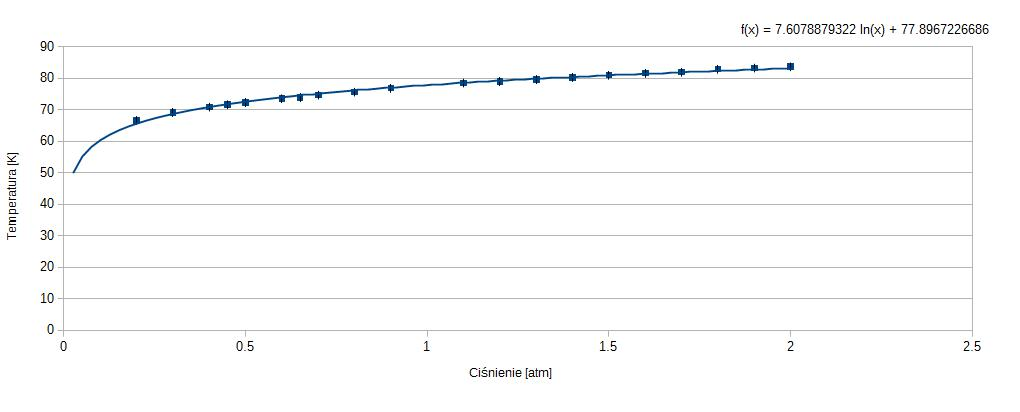
\includegraphics[scale=0.51]{ch01}
\caption{Wykres zależności temperatur wrzenia od ciśnienia}
\end{figure}

\subsection{Obliczenie wartości ciepła parowania pod ciśnieniem atmosferycznym}

Równanie Clausiusa-Clapeyrona ma postać:
\begin{equation}
	\frac{dT}{dp} = \frac{T(V_{2}-V_{1})}{Q}
\end{equation}

gdzie:
Q - ciepło przemiany \\
T - temperatura przejścia \\
$\frac{dT}{dp}$ - pochodna zależności temperatury przejścia od ciśnienia \\ 
$V_{2}-V_{1}$ - różnica objętości faz

Objętość właściwą azotu ciekłego otrzymujemy natychmiast z zależności:
\begin{equation}
	V_1 = \frac{m}{\rho} = \frac{1000 g}{0.808 \frac{g}{cm^3}} \approx 1238 cm^3
\end{equation}

Objętość właściwa azotu w stanie gazowym została wyliczona z równania stanu gazu doskonałego przekształconego do postaci:
\begin{equation}
	V_2 = \frac{mRT}{Mp} = \frac{1000 g \cdot 8.31 \frac{J}{mol \cdot K } \cdot 77.3K}{28 \frac{g}{mol} \cdot 1.02 \cdot 10^5 Pa} \approx 0.225 m^3
\end{equation}

Natomiast wartość pochodnej $\frac{dT}{dp}$ wyznaczymy analitycznie:\\
Mając do dyspozycji wzór regresji logarytmicznej f(x) = 7.6079 ln(x) - 	9.793. Obliczamy pochodną z funkcji: f'(x) = $\frac{7.6079}{x}$, która w punkcie x = 101325 Pa (dla p = 1 atm) wynosi 7.51 $\cdot 10^{-5}$ $\frac{K}{Pa}$

Teraz pozostaje rozwiązać równanie (1):
\begin{equation}
	Q = T(V_2-V_1) \cdot \frac{1}{\frac{dT}{dp}} = 77.3K \cdot (0.225 m^3 - 0.001238 m^3) \cdot \frac{1}{7.51 \cdot 10^{-5} \frac{K}{Pa}} = 2.303 \cdot 10^{5} \frac{J}{kg} = 230.3 \frac{J}{g}
\end{equation}

\subsection{Pomiar ciepła parowania}
Na początku obliczmy masę słupa o wysokości wybranej przez nas: $\Delta h = 70 mm$:

\begin{equation}
	m = V \cdot \rho = 49.5 cm^3 \cdot 0.000808 \frac{g}{cm^3} \approx 40.0 \:g
\end{equation}

By obliczyć ciepło parowania należy rozwiązań następujący układ równań:
\begin{equation}
	\begin{cases}
	P_s t_1 = \Delta m_1 Q_p \\
	(P_s + P) \cdot t_2 = \Delta m_2 Q_p
	\end{cases}
\end{equation}

W naszym przypadku $\Delta m_1$ oraz $\Delta m_2$ to ta sama wartość wyliczona powyżej.

Po przekształceniach i wstawieniu danych uzyskanych w drugiej części eksperymentu otrzymujemy $Q_p = 126 \frac{J}{g}$
%----------------------------------------------------------------------------------------
%	SECTION 6
%----------------------------------------------------------------------------------------
\section{Wnioski}


%----------------------------------------------------------------------------------------
%	BIBLIOGRAPHY
%----------------------------------------------------------------------------------------

\bibliographystyle{apalike}

\bibliography{sample}
%----------------------------------------------------------------------------------------


\end{document}
